\chapter{Fonctions affines}

\section{Définitions et représentations graphiques}

\subsection{Fonctions affines, particulières et contre-exemples}

\begin{defin}[Fonction affine]
	Soit $f$ une fonction définie sur $\mathbb{R}$.

	$f$ est une \textbf{fonction affine} s'il existe deux réels $m$ et $p$ tels que, pour tout $x \in \mathbb{R}$ :

	\[
		f(x) = \textcolor{red}{m}x + \textcolor{blue}{p}
	\]

	Le réel $\textcolor{red}{m}$ est appelé le \textbf{coefficient directeur} (ou la pente) et $\textcolor{blue}{p}$ est l' \textbf{ordonnée à l'origine}.
\end{defin}

\begin{defin}[Cas particuliers]
	Soit $f(x) = mx + p$ une fonction affine :

	\begin{itemize}
		\item Si $p = 0$, $f(x) = mx$. La fonction $f$ est dite \textbf{linéaire}.

		      Elle traduit une situation de proportionnalité.
		\item Si $m = 0$, $f(x) = p$. La fonction $f$ est dite \textbf{constante}.
	\end{itemize}
\end{defin}

\begin{ex}
	\nline
	\begin{center}
		\def\arraystretch{1.5}
		\begin{tabular}{|l|c|c|l|} \hline
			\textbf{Fonction}                                                                & $\textcolor{red}{m}$ & $\textcolor{blue}{p}$ & \textbf{Nature}                \\ \hline
			$f(x) = 3x - 4$                                                                  & $3$                  & $-4$                  & Fonction affine                \\ \hline
			$g(x) = -x + 2$                                                                  & $-1$                 & $2$                   & Fonction affine                \\ \hline
			$h(x) = 5x$                                                                      & $5$                  & $0$                   & Fonction linéaire (et affine)  \\ \hline
			$k(x) = -7$                                                                      & $0$                  & $-7$                  & Fonction constante (et affine) \\ \hline
			\rule[-5mm]{0mm}{13mm}$l(x) = \dfrac{1 - 2x}{3} = -\dfrac{2}{3}x + \dfrac{1}{3}$ & $-\dfrac{2}{3}$      & $\dfrac{1}{3}$        & Fonction affine                \\ \hline
		\end{tabular}
	\end{center}
\end{ex}

\begin{rem}
	\textbf{Contre-exemples :} $x \mapsto x^2 + 1$, $x \mapsto \dfrac{2}{x}$ ou $x \mapsto \sqrt{x}$ ne sont pas des fonctions affines.
\end{rem}

\subsection{Représentation graphique}

\begin{prop}{}
	Dans un repère, la représentation graphique de la fonction affine $f(x) = mx + p$ est une \textbf{droite} non verticale, notée $\mathcal{D}_f$.
	\begin{itemize}
		\item Un point $M(x\,;\,y)$ appartient à $\mathcal{D}_f$ si et seulement si $y = f(x) = mx + p$.
		\item $p$ est l'ordonnée du point d'intersection de $\mathcal{D}_f$ avec l'axe des ordonnées : la droite passe par $(0\,;\,p)$.
		\item Si $f$ est linéaire ($p = 0$), la droite passe par l'origine $O(0\,;\,0)$.
		\item Si $f$ est constante ($m = 0$), la droite est horizontale.
	\end{itemize}
\end{prop}

\newpage

\begin{methode}[Lire graphiquement $m$ et $p$]
	\nline
	\begin{wrapstuff}[r]
		\begin{tikzpicture}[scale=0.8]
			\draw[very thin, gray!40] (-1.5,-2.5) grid (4.5,4.5);
			\draw[-{Stealth}, black, thick] (-1.5,0) -- (4.5,0) node[right] {$x$};
			\draw[-{Stealth}, black, thick] (0,-2.5) -- (0,4.5) node[above] {$y$};
			\foreach \x in {-1,1,2,3,4} \node[below, font=\tiny, black] at (\x,0) {\x};
			\foreach \y in {-2,-1,1,2,3,4} \node[left, font=\tiny, black] at (0,\y) {\y};
			\node[below left, font=\tiny] at (0,0) {0};
			\node[right=2pt, font=\small, fill=white, anchor=north west] at (0,-1) {$(0\,;\, - 1)$};
			\draw[blue, ultra thick, domain=-1.1:3.5] plot(\x,{1.5*\x - 1});
			\filldraw[blue] (0,-1) circle (2pt);
			\node[green!50!black, below, font=\small, fill=white] at (2,0.2) {$\Delta x = +2$} ;
			\draw[green!50!black, thick, dashed] (1,0.5) -- (3,0.5) -- (3,3.5);
			\draw[green!50!black, thick, <->] (1,0.2) -- (3,0.2);
			\draw[green!50!black, thick, <->] (3.2,0.5) -- node[right, font=\small, fill=white] {$\Delta y = +3$} (3.2,3.5);
			\node[above left, font=\small,fill=white] at (1,0.5) {$A(1\,;\,0{,}5)$};
			\filldraw[red] (1,0.5) circle (3pt);
			\node[above left, font=\small,fill=white] at (3,3.5) {$B(3\,;\,3{,}5)$};
			\filldraw[red] (3,3.5) circle (3pt);
		\end{tikzpicture}
	\end{wrapstuff}

	Pour lire l'expression de la fonction affine associée à la droite ci-contre :

	\begin{enumerate}
		\item \textbf{Ordonnée à l'origine :}

		      La droite coupe l'axe des ordonnées au point $(0\,;\, - 1)$, donc $\textcolor{blue}{p = -1}$.
		\item \textbf{Coefficient directeur :}

		      On choisit deux points $A(1\,;\,0{,}5)$ et $B(3\,;\,3{,}5)$.

		      En passant de $A$ à $B$, on avance de $\Delta x = 2$ et on monte de $\Delta y = 3$.

		      Ainsi :
		      \[
			      {m} = \frac{\Delta y}{\Delta x} = \frac{3{,}5 - 0{,}5}{3 - 1} = \frac{3}{2} = 1{,}5
		      \]
	\end{enumerate}

	On en déduit que :
	\[
		f(x) = 1{,}5x - 1
	\]
\end{methode}

\section{Propriétés analytiques et variations}

\subsection{Taux d'accroissement}

\begin{prop}[Taux d'accroissement]
	Soit $f$ une fonction affine $f(x) = mx + p$. Pour tous réels $a$ et $b$ distincts ($a \neq b$) :
	\[
		m = \frac{f(b) - f(a)}{b - a}
	\]

	Le coefficient directeur mesure \textbf{le taux de variation} constant de la fonction.
\end{prop}

\begin{methode}[Déterminer une fonction affine à partir de deux points ou images]
	Déterminer la fonction affine $f$ telle que $f(-1) = 3$ et $f(5) = 1$.

	\begin{correction}
		\nline
		\begin{enumerate}
			\item On calcule le coefficient directeur $m$ :
			      \[
				      \textcolor{red}{m} = \frac{f(5) - f(-1)}{5 - (-1)} = \frac{1 - 3}{5 + 1} = \frac{-2}{6} = \textcolor{red}{-\frac{1}{3}}
			      \]

			      Ainsi, $f(x) = \dfrac{-1}{3}x + p$.
			\item On détermine $p$ en utilisant l'une des deux images, par exemple $f(5) = 1$ :
			      \[
				      f(5) = 1 \iff -\frac{1}{3} \times 5 + p = 1 \iff -\frac{5}{3} + p = 1 \iff p = 1 + \frac{5}{3} = \textcolor{blue}{\frac{8}{3}}
			      \]
		\end{enumerate}

		L'expression cherchée est donc $f(x) = \dfrac{-1}{3}x + \dfrac{8}{3}$.
	\end{correction}
\end{methode}

\newpage

\subsection{Sens de variation}

\begin{prop}[Variations d'une fonction affine]
	Soit $f(x) = mx + p$ définie sur $\mathbb{R}$.
	\begin{itemize}
		\item Si $m > 0$, $f$ est \textbf{strictement croissante} sur $\mathbb{R}$.
		\item Si $m < 0$, $f$ est \textbf{strictement décroissante} sur $\mathbb{R}$.
		\item Si $m = 0$, $f$ est \textbf{constante} sur $\mathbb{R}$.
	\end{itemize}
\end{prop}

\begin{ex}[Variation d'une fonction affine]
	Soit $f(x) = -3x + 5$ définie sur $\mathbb{R}$.\par

	On a $m = -3 < 0$, donc $f$ est \textbf{strictement décroissante} sur $\mathbb{R}$.

	\begin{center}
		\begin{tikzpicture}
			\tkzTabInit[lgt=2, espcl=3]{$x$ / 0.5, $f(x)$ / 1}{$-\infty$, $+\infty$}
			\tkzTabVar{+ / , - / }
		\end{tikzpicture}
	\end{center}
\end{ex}

\subsection{Signe de $f(x) = mx + p$}

\begin{prop}[Tableau de signe]
	La fonction affine $f(x) = mx + p$ avec $m \neq 0$ s'annule en $x = \dfrac{-p}{m}$.

	Cette valeur est appelée la \textbf{racine} de la fonction.

	Son signe dépend du signe de son coefficient directeur $m$ (\textbf{signe de $m$ à droite du zéro}) :

	\begin{center}
		\def\arraystretch{1.5}
		\begin{tabular}{cc}
			Si $m > 0$ & Si $m < 0$ \\[4pt]
			\begin{tikzpicture}
				\tkzTabInit[lgt=1.5, espcl=2]{$x$/1, $f(x)$/1}{$-\infty$, $\frac{-p}{m}$, $+\infty$}
				\tkzTabLine{,-,z,+,}
			\end{tikzpicture}
			           &
			\begin{tikzpicture}
				\tkzTabInit[lgt=1.5, espcl=2]{$x$/1, $f(x)$/1}{$-\infty$, $\frac{-p}{m}$, $+\infty$}
				\tkzTabLine{,+,z,-,}
			\end{tikzpicture}
		\end{tabular}
	\end{center}
\end{prop}

\begin{meth}[Étude complète du signe]
	Déterminer le signe de $g(x) = -2x + 6$ sur $\mathbb{R}$.
	\begin{correction}
		\nline
		\begin{itemize}
			\item \textbf{Racine :}
			      \begin{align*}
				      g(x) = 0 & \iff -2x + 6 = 0 \\
				               & \iff -2x = -6    \\
				               & \iff x = 3
			      \end{align*}
			\item \textbf{Signe :}

			      $m = -2 < 0$, donc $g(x)$ est positive avant 3 puis négative après.
		\end{itemize}
		\begin{center}
			\begin{tikzpicture}
				\tkzTabInit[lgt=1.5, espcl=2]{$x$/1, $g(x)$/1}{$-\infty$, $3$, $+\infty$}
				\tkzTabLine{,+,z,-,}
			\end{tikzpicture}
		\end{center}
	\end{correction}
\end{meth}

\newpage

\section{Applications : Inéquations produit et quotient}

Le tableau de signe des fonctions affines permet de résoudre des inéquations plus complexes par la règle des signes.

\begin{methode}[Inéquation produit]
	Résoudre sur $\mathbb{R}$ l'inéquation $(3x - 1)(2 - x) \ge 0$.

	\begin{correction}
		\nline
		\begin{enumerate}
			\item \textbf{Recherche des racines :}
			      \begin{itemize}
				      \item $3x - 1 = 0 \iff x = \dfrac{1}{3}$ \quad (avec $m = 3 > 0$)
				      \item $2 - x = 0 \iff x = 2$ \quad (avec $m = -1 < 0$)
			      \end{itemize}
			\item \textbf{Tableau de signe synthétique :}
			      \begin{center}
				      \begin{tikzpicture}
					      \tkzTabInit[lgt=3.5, espcl=2]
					      {$x$/1, $3x - 1$/1, $2 - x$/1, $(3x - 1)(2 - x)$/1}
					      {$-\infty$, $\dfrac{1}{3}$, $2$, $+\infty$}
					      \tkzTabLine{,-,z,+,t,+,}
					      \tkzTabLine{,+,t,+,z,-,}
					      \tkzTabLine{,-,z,+,z,-,}
				      \end{tikzpicture}
			      \end{center}
			\item \textbf{Conclusion :} On cherche les valeurs où le produit est supérieur ou égal à 0.
			      \[
				      S = \intff{\frac{1}{3}}{2}
			      \]
		\end{enumerate}
	\end{correction}
\end{methode}

\begin{methode}[Inéquation quotient]
	Résoudre sur $\mathbb{R}$ l'inéquation $\dfrac{4x + 2}{1 - x} < 0$.

	\begin{correction}
		\nline
		\begin{enumerate}
			\item \textbf{Valeur interdite :} $1 - x = 0 \iff x = 1$. L'ensemble de définition est $\mathbb{R} \setminus \{1\}$.
			\item \textbf{Racine du numérateur :} $4x + 2 = 0 \iff x = -\dfrac{1}{2}$.
			\item \textbf{Tableau de signe (avec double barre pour la valeur interdite) :}
			      \begin{center}
				      \begin{tikzpicture}
					      \tkzTabInit[lgt=3.5, espcl=2]
					      {$x$/1, $4x + 2$/1, $1 - x$/1, $\dfrac{4x+2}{1-x}$/1}
					      {$-\infty$, $-\dfrac{1}{2}$, $1$, $+\infty$}
					      \tkzTabLine{,-,z,+,t,+,}
					      \tkzTabLine{,+,t,+,z,-,}
					      \tkzTabLine{,-,z,+,d,-,}
				      \end{tikzpicture}
			      \end{center}
			\item \textbf{Conclusion :} On cherche le signe strictement négatif ($< 0$).
			      \[
				      S = \left] -\infty\,;\, - \frac{1}{2} \right[\  \cup \ \left] 1\,;\, + \infty \right[
			      \]
		\end{enumerate}
	\end{correction}
\end{methode}


